% (C) Brett Klamer - MIT - http://opensource.org/licenses/MIT
% Please contact me if you find any errors or make improvements
% Contact details at brettklamer.com

\documentclass[11pt,letterpaper,english,oneside]{article}\usepackage[]{graphicx}\usepackage[]{color}
% maxwidth is the original width if it is less than linewidth
% otherwise use linewidth (to make sure the graphics do not exceed the margin)
\makeatletter
\def\maxwidth{ %
  \ifdim\Gin@nat@width>\linewidth
    \linewidth
  \else
    \Gin@nat@width
  \fi
}
\makeatother

\definecolor{fgcolor}{rgb}{0.345, 0.345, 0.345}
\newcommand{\hlnum}[1]{\textcolor[rgb]{0.686,0.059,0.569}{#1}}%
\newcommand{\hlstr}[1]{\textcolor[rgb]{0.192,0.494,0.8}{#1}}%
\newcommand{\hlcom}[1]{\textcolor[rgb]{0.678,0.584,0.686}{\textit{#1}}}%
\newcommand{\hlopt}[1]{\textcolor[rgb]{0,0,0}{#1}}%
\newcommand{\hlstd}[1]{\textcolor[rgb]{0.345,0.345,0.345}{#1}}%
\newcommand{\hlkwa}[1]{\textcolor[rgb]{0.161,0.373,0.58}{\textbf{#1}}}%
\newcommand{\hlkwb}[1]{\textcolor[rgb]{0.69,0.353,0.396}{#1}}%
\newcommand{\hlkwc}[1]{\textcolor[rgb]{0.333,0.667,0.333}{#1}}%
\newcommand{\hlkwd}[1]{\textcolor[rgb]{0.737,0.353,0.396}{\textbf{#1}}}%
\let\hlipl\hlkwb

\usepackage{framed}
\makeatletter
\newenvironment{kframe}{%
 \def\at@end@of@kframe{}%
 \ifinner\ifhmode%
  \def\at@end@of@kframe{\end{minipage}}%
  \begin{minipage}{\columnwidth}%
 \fi\fi%
 \def\FrameCommand##1{\hskip\@totalleftmargin \hskip-\fboxsep
 \colorbox{shadecolor}{##1}\hskip-\fboxsep
     % There is no \\@totalrightmargin, so:
     \hskip-\linewidth \hskip-\@totalleftmargin \hskip\columnwidth}%
 \MakeFramed {\advance\hsize-\width
   \@totalleftmargin\z@ \linewidth\hsize
   \@setminipage}}%
 {\par\unskip\endMakeFramed%
 \at@end@of@kframe}
\makeatother

\definecolor{shadecolor}{rgb}{.97, .97, .97}
\definecolor{messagecolor}{rgb}{0, 0, 0}
\definecolor{warningcolor}{rgb}{1, 0, 1}
\definecolor{errorcolor}{rgb}{1, 0, 0}
\newenvironment{knitrout}{}{} % an empty environment to be redefined in TeX

\usepackage{alltt} % article class is a standard class
%==============================================================================
%Load Packages
%==============================================================================
\usepackage[left=1in,right=1in,top=1in,bottom=1in]{geometry} % easy page margins
\usepackage[utf8]{inputenc} % editor uses utf-8 encoding
\usepackage[T1]{fontenc} % T1 font pdf output
\usepackage{lmodern} % Latin modern roman font
\usepackage{bm, bbm} % bold and blackboard bold math symbols
\usepackage{amsmath, amsfonts, amssymb, amsthm} % math packages
\usepackage[final]{microtype} % better microtypography
\usepackage{graphicx} % for easier grahics handling
\usepackage[hidelinks, colorlinks=true, linkcolor = blue, urlcolor = blue]{hyperref} % to create hyperlinks
\usepackage{float} % tells floats to stay [H]ere!
\usepackage{mdframed} % it's better than framed. knitr uses framed so settings won't conflict
\usepackage{enumitem} % nice lists
\usepackage{fancyhdr} % nice headers
\usepackage{caption}  % to control figure and table captions

\captionsetup{width=0.9\textwidth, justification = raggedright}

%==============================================================================
% Enter name and homework title here
%==============================================================================
\author{Jiahang Sha}
\title{STAT 961: Homework 4}
\date{Due Friday, November 19 at 11:59pm}

%==============================================================================
% Put title and author in PDF properties
%==============================================================================
\makeatletter % change interpretation of @
\hypersetup{pdftitle={\@title},pdfauthor={\@author}}


%==============================================================================
% Header settings
%==============================================================================
\pagestyle{fancy} % turns on fancy header styles
\fancyhf{} % clear all header and footer fields
\makeatletter
\lhead{\@author} % left header
\chead{\@title} % center header
\makeatother
\rhead{Page \thepage} % right header
\setlength{\headheight}{13.6pt} % fixes minor warning
\makeatother % change back interpretation of @

%==============================================================================
% List spacing
%==============================================================================
\setlist[itemize]{parsep=0em} % fix itemize spacing
\setlist[enumerate]{parsep=0em} % fix enumerate spacing

%==============================================================================
% Float spacing (changes spacing of tables, graphs, etc)
%==============================================================================
%\setlength{\textfloatsep}{3pt}
%\setlength{\intextsep}{3pt}

%==============================================================================
% Define Problem and Solution Environments
%==============================================================================
\theoremstyle{definition} % use definition's look
\newtheorem{problem}{Problem}
\newtheorem{solution}{Solution}
\mdfsetup{ % box margin fix for mdframe and how it plays with parskip and others.
innerleftmargin=4pt,
innerrightmargin=4pt,
innertopmargin=-1pt,
innerbottommargin=4pt}
% \newenvironment{prob}{\begin{mdframed}\begin{problem}\hspace{0pt}}{\end{problem}\end{mdframed}}
\newenvironment{prob}{\clearpage \begin{problem}\hspace{0pt}}{\end{problem}}
\newenvironment{sol}{\begin{solution}\hspace{0pt}}{\end{solution}}

%==============================================================================
% set knitr options
%==============================================================================
% latex (change space before and after knitr kframe; based on framed package)
\setlength{\OuterFrameSep}{0.3em}
% R


\IfFileExists{upquote.sty}{\usepackage{upquote}}{}
\begin{document}


\maketitle

\section{Instructions}

\paragraph{Setup.} Pull the latest version of this assignment from Github and set your working directory to \texttt{stat-961-fall-2021/homework/homework-4}. Consult the \href{https://github.com/Katsevich-Teaching/stat-961-fall-2021/blob/main/getting-started/getting-started.pdf}{getting started guide} if you need to brush up on \texttt{R}, \texttt{LaTeX}, or \texttt{Git}.

\paragraph{Collaboration.} The collaboration policy is as stated on the Syllabus:

\begin{quote}
``Students are permitted to work together on homework assignments, but solutions must be written up and submitted individually. Students must disclose any sources of assistance they received; furthermore, they are prohibited from verbatim copying from any source and from consulting solutions to problems that may be available online and/or from past iterations of the course.''
\end{quote}

\noindent In accordance with this policy, \\

\noindent \textit{Please list anyone you discussed this homework with:} Professor Katsevich, Wenshuo Liu, Sam Rosenberg\\

\noindent \textit{Please list what external references you consulted (e.g. articles, books, or websites):} uniroot, ggplot documentation\\

\paragraph{Writeup.} Use this document as a starting point for your writeup, adding your solutions between \verb|\begin{sol}| and \verb|\end{sol}|. See the \href{https://github.com/Katsevich-Teaching/stat-961-fall-2021/blob/main/getting-started/preparing-reports.pdf}{preparing reports guide} for guidance on compilation, creation of figures and tables, and presentation quality. Show all the code you wrote to produce your numerical results, and include complete derivations typeset in LaTeX for the mathematical questions. 

\paragraph{Programming.}

The \texttt{tidyverse} paradigm for data manipulation (\texttt{dplyr}) and plotting (\texttt{ggplot2}) are strongly encouraged, but points will not be deducted for using base \texttt{R}. 
\begin{knitrout}
\definecolor{shadecolor}{rgb}{0.969, 0.969, 0.969}\color{fgcolor}\begin{kframe}
\begin{alltt}
\hlkwd{library}\hlstd{(tidyverse)}
\end{alltt}
\end{kframe}
\end{knitrout}

\paragraph{Grading.} Each sub-part of each problem will be worth 3 points: 0 points for no solution or completely wrong solution; 1 point for some progress; 2 points for a mostly correct solution; 3 points for a complete and correct solution modulo small flaws. The presentation quality of the solution for each problem (as exemplified by the guidelines in Section 3 of the \href{https://github.com/Katsevich-Teaching/stat-961-fall-2021/blob/main/getting-started/preparing-reports.pdf}{preparing reports guide}) will be evaluated out of an additional 3 points.

\paragraph{Submission.} Compile your writeup to PDF and submit to \href{https://www.gradescope.com/courses/284562}{Gradescope}.

\clearpage

\begin{prob} \label{prob:ci-calculation}\textbf{Inverting the Wald, likelihood ratio, and score tests for a Poisson GLM.} \\

\noindent You have two email accounts: your personal one and your academic one. Last month, you received $y_1$ and $y_2$ emails in your personal and academic inboxes, respectively. Interested in the extent to which you receive more (or less) email in your academic inbox, you set up the following Poisson regression model:
\begin{equation*}
y_i \overset{\text{ind}} \sim \text{Poi}(\mu_i); \quad \log \mu_i = \beta_0 + \beta_1 x_i; \quad i \in \{1,2\},
\end{equation*}
where $x_i \in \{0,1\}$ is an indicator for your academic inbox. Your goal is to build a level-$\alpha$ confidence interval for $e^{\beta_1}$ (the factor by which the expected number of emails in your academic inbox exceeds that in your personal inbox), and to this end you will invert the Wald, likelihood ratio, and score tests.

\begin{enumerate}

\item[(a)] What is the unrestricted maximum likelihood estimate $(\widehat \beta_0, \widehat \beta_1)$? What are the corresponding fitted means $(\widehat \mu_1, \widehat \mu_2)$? What is the maximum likelihood estimate for $\beta_0$ if $\beta_1$ is fixed at some value $\beta_1^0 \in \mathbb R$? What are the corresponding fitted means? What do the fitted means reduce to when $\beta_1^0 = 0$, and why does this make sense?

\item[(b)] What is the large-sample normal approximation to the sampling distribution of $\bm{\widehat \beta}$? What is the resulting level-$\alpha$ Wald confidence interval for $e^{\beta_1}$ (defined by transforming the endpoints of the Wald confidence interval for $\beta_1$)? Express your answer explicitly.

\item[(c)] Given some $\beta_1^0 \in \mathbb R$, what is the likelihood ratio test statistic for $H_0: \beta_1 = \beta_1^0$? What is the level-$\alpha$ confidence interval for $e^{\beta_1}$ that results from inverting this test? The endpoints of your interval may be specified as solutions to a nonlinear equation.

\item[(d)] Formulate the test $H_0: \beta_1 = \beta_1^0$ as a goodness of fit test. What is the corresponding score test statistic? What is the level-$\alpha$ confidence interval for $e^{\beta_1}$ that results from inverting this test? Express your answer explicitly.


\end{enumerate}

\end{prob}

\begin{sol}
\begin{enumerate}
    \item[a.]
    $\log \mathcal L(\bm \beta) = \sum_{i = 1}^n (\theta_i y_i - \psi(\theta_i)) + \sum_{i = 1}^n \log h(y_i) 
    = \beta_0y_1 - e^{\beta_0} + (\beta_0+\beta_1)y_2 - e^{\beta_0+\beta_1}  - \log(y_1!) -\log(y_2!).$    Taking gradients, we get $\nabla \log \mathcal L(\bm \beta) =
    \begin{bmatrix}
    y_1-e^{\beta_0} + y_2 - e^{\beta_0+\beta_1} \\
    y_2 - e^{\beta_0+\beta_1}
    \end{bmatrix}$. Setting this to be 0, we get $\hat{\beta}_0 = \log(y_1), \hat{\beta}_1 = \log(\frac{y_2}{y_1}).$ The corresponding fitted values means $(\hat{\mu}_1, \hat{\mu}_2) = e^{X\beta}= (y_1, y_2)$.\\
    
    Suppose $\beta_1^0$ is fixed. Then, we compute $\nabla_{\beta_0} \log \mathcal L(\bm \beta) =y_1-e^{\beta_0} + y_2 - e^{\beta_0+\beta_1^0}$. Setting this to be 0, we get $\hat{\beta}_0 = \log(\frac{y_1+y_2}{1+e^{\beta_1^0}}).$    In this case, the corresponding fitted means $(\hat{\mu}_1, \hat{\mu}_2) = (\frac{y_1+y_2}{1+e^{\beta_1^0}}, e^{\beta_1^0}\frac{y_1+y_2}{1+e^{\beta_1^0}})$.\\
    
    When $\beta_1^0$ is fixed to be 0, we compute $(\hat{\mu}_1, \hat{\mu}_2) = (\frac{y_1+y_2}{1+e^{0}}, e^{0}\frac{y_1+y_2}{1+e^{0}})=(\frac{y_1+y_2}{2}, \frac{y_1+y_2}{2})$. This assumption means that the indicator is assumed to not work, and therefore no difference in the number of incoming emails between two mailboxes is assumed. Two email boxes have the same probability to receive an email, so the fitted means should of course be the average of the total number of emails I received.
    \item[(b)]
    $I(\beta) = -E[\nabla^2 \log \mathcal L(\bm \beta)] =
    \begin{bmatrix}
    e^{\beta_0}+ e^{\beta_0+\beta_1} &  e^{\beta_0+\beta_1}\\
     e^{\beta_0+\beta_1} &  e^{\beta_0+\beta_1}
    \end{bmatrix}$. Plugging in $\hat{\beta}$, we derive $I(\hat{\beta}) =
    \begin{bmatrix}
    y_1+ y_2 &  y_2\\
     y_2 &  y_2
    \end{bmatrix}$. Therefore, $I(\hat{\beta})^{-1} = \begin{bmatrix}
    \frac{1}{y_1}&  -\frac{1}{y_1}\\
    - \frac{1}{y_1} &  \frac{y_1+y_2}{y_1y_2}
    \end{bmatrix}$. We use (39) and (40) $\hat{\beta} \sim N(\beta, \begin{bmatrix}
    \frac{1}{y_1}&  -\frac{1}{y_1}\\
    - \frac{1}{y_1} &  \frac{y_1+y_2}{y_1y_2}
    \end{bmatrix})$, where $\hat{\beta_1} \sim N(\beta_1,  \frac{y_1+y_2}{y_1y_2})$. We use (41) to construct \\
    $$\text{CI}(\hat{\beta}_1) = \left[\log(\frac{y_2}{y_1})- z_{1-\alpha/2}\sqrt{\frac{y_1+y_2}{y_1y_2}} ,\log(\frac{y_2}{y_1})+z_{1-\alpha/2}\sqrt{\frac{y_1+y_2}{y_1y_2}}\right] $$
    
    Applying $e^x$ to the obtained confidence interval, we find \\
    $$\text{CI}(e^{\hat{\beta}_1}) = \left[\frac{y_2}{y_1}e^{-z_{1-\alpha/2}\sqrt{\frac{y_1+y_2}{y_1y_2}}}, \frac{y_2}{y_1} e^{z_{1-\alpha/2}\sqrt{\frac{y_1+y_2}{y_1y_2}}} \right]$$
    all at a confidence level $\alpha$.
    
    \item[(c)]
    By (37) we know the deviance for Poisson GLMs with log-link $D(y;\hat{\mu}) = 2(y_1\log(y_1/\hat{\mu}_1) +y_2\log(y_2/\hat{\mu}_2))=0$\\
    and $D(y;\hat{\mu}_{-S}) = 2(y_1\log(y_1/\hat{\mu}_1^0) +y_2\log(y_2/\hat{\mu}_2^0))=2\left(y_1 \log\left(\frac{(e^{\beta_1^0}+1)y_1 }{y_1 +y_2 }\right)+y_2 \log\left(\frac{(e^{\beta_1^0}+1)y_2 }{e^{\beta_1^0}(y_1 +y_2 )}\right)\right)$. In this model, $|S|=1$. Therefore, we use LRT test statistics in terms of difference in deviances $$T^{LRT} = D(y;\hat{\mu}_{-S})- D(y;\hat{\mu})=2\left(y_1 \log\left(\frac{(e^{\beta_1^0}+1)y_1 }{y_1 +y_2 }\right)+y_2 \log\left(\frac{(e^{\beta_1^0}+1)y_2 }{e^{\beta_1^0}(y_1 +y_2 )}\right)\right)\sim \chi^2_1$$.  \\
    Therefore, CI$(e^{\beta_1}) = \{x:2\left(y_1 \log\left(\frac{(x+1)y_1 }{y_1 +y_2 }\right)+y_2 \log\left(\frac{(x+1)y_2 }{x(y_1 +y_2 )}\right)\right) \leq \chi^2_{1,1-\alpha}\} \\
    = \{x: (y_1+y_2)\log(1+x) - y_2 \log(x) \leq \frac{\chi^2_{1,1-\alpha}}{2}-y_1 \log(\frac{y_1}{y_1+y_2}) - y_2 \log(\frac{y_2}{y_1+y_2})\}$.
    \item[(d)]
    Under $H_0$, we have $(\hat{\mu}_1, \hat{\mu}_2) = (\frac{y_1+y_2}{1+e^{\beta_1^0}}, e^{\beta_1^0}\frac{y_1+y_2}{1+e^{\beta_1^0}})$. Therefore, the score test statistic is $$\frac{(y_1-\hat{\mu}_1)^2}{\hat{\mu}_1}+\frac{(y_2-\hat{\mu}_2)^2}{\hat{\mu}_2}=\frac{(y_1-\frac{y_1+y_2}{1+e^{\beta_1^0}})^2}{\frac{y_1+y_2}{1+e^{\beta_1^0}}}+\frac{(y_2-e^{\beta_1^0}\frac{y_1+y_2}{1+e^{\beta_1^0}})^2}{e^{\beta_1^0}\frac{y_1+y_2}{1+e^{\beta_1^0}}}=\frac{(y_2-y_1e^{\beta_1^0)^2}}{(y_1+y_2)e^{\beta_1^0}}\sim \chi^2_1$$
    Inverting this test, we solve the quadratic inequality and obtain the confidence interval as 
    $$\text{CI}(e^{\beta_1}) = \left[\frac{\chi^2_{1, (1-\alpha)} y_1 +\chi^2_{1, (1-\alpha)} y_2 +2y_1 y_2 -\sqrt{c_1}}{2y_1 ^2},\frac{\chi^2_{1, (1-\alpha)} y_1 +\chi^2_{1, (1-\alpha)} y_2 +2y_1 y_2 +\sqrt{c_1}}{2y_1 ^2}\right]$$
    where $c_1 = \chi^2_{1, (1-\alpha)} ^2y_1 ^2+2\chi^2_{1, (1-\alpha)} ^2y_1 y_2+\chi^2_{1, (1-\alpha)} ^2y_2 ^2+4\chi^2_{1, (1-\alpha)} y_1 ^2y_2 +4\chi^2_{1, (1-\alpha)} y_1 y_2 ^2$.
\end{enumerate}
\end{sol}

\begin{prob} \label{prob:ci-simulation}\textbf{Comparing the three confidence interval constructions from Problem~\ref{prob:ci-calculation}.} \\

\noindent Let's use a numerical simulation to compare the three confidence interval constructions from Problem~\ref{prob:ci-calculation} in finite samples.

\begin{enumerate}

\item[(a)] Write functions called \verb|get_ci_wald|, \verb|get_ci_lrt|, and \verb|get_ci_score| that take as arguments (\verb|y_1|, \verb|y_2|, \verb|alpha|) and return the corresponding confidence intervals for $e^{\beta_1}$. If the confidence interval is undefined for a given pair $(y_1, y_2)$, your function should return $(-\infty, \infty)$.

\item[(b)] To get a first sense of how the three intervals compare, compute level $\alpha = 0.05$ intervals for $(y_1, y_2) = (10^1, 10^1), (10^{1.5}, 10^{1.5}), \dots, (10^5, 10^5)$. Plot the lower and upper endpoints of these intervals as functions of $y_1$ (you should arrive at a plot containing six curves, corresponding to the lower and upper endpoints of the three methods). Add a dashed horizontal line at the MLE for $e^{\beta_1}$ (which is the same for each given pair $(y_1, y_2)$). How do the interval widths compare, both across methods and across $(y_1, y_2)$ values?

\item[(c)] Next, calculate the average length and coverage of the three level $\alpha = 0.05$ confidence intervals for $e^{\beta_1}$ in the following simulation setting. Set $(\mu_1, \mu_2) = (10^1, 10^1), (10^{1.5}, 10^{1.5}), \dots, (10^5, 10^5)$. For each pair $(\mu_1, \mu_2)$, generate 5000 realizations of $(y_1, y_2)$ and compute the three confidence intervals for each realization. Plot the average length and coverage for each of the three interval constructions as a function of $\mu_1$ (please omit the undefined/infinite-length intervals from the calculations of length and coverage). Compare and contrast the average lengths and coverages of the three constructions, both across methods and across $(\mu_1, \mu_2)$ values.

\item[(d)] Last month you received 60 emails in your personal inbox and 90 in your academic inbox. Pick one of the three confidence interval constructions above that you feel has good coverage and small width. According to this construction, what is the confidence interval for $e^{\beta_1}$? Can you reject the null hypothesis that the two inboxes receive emails at the same rate?
\end{enumerate}


\end{prob}

\begin{sol}
\begin{enumerate}
\item[(a)]
\begin{knitrout}
\definecolor{shadecolor}{rgb}{0.969, 0.969, 0.969}\color{fgcolor}\begin{kframe}
\begin{alltt}
\hlcom{#function to return return CI by wald test}
\hlstd{get_ci_wald} \hlkwb{<-} \hlkwa{function}\hlstd{(}\hlkwc{y_1}\hlstd{,} \hlkwc{y_2}\hlstd{,} \hlkwc{alpha}\hlstd{)\{}
  \hlstd{df} \hlkwb{=} \hlkwd{data.frame}\hlstd{(}\hlstr{'lower'} \hlstd{=} \hlopt{-}\hlnum{Inf}\hlstd{,} \hlstr{'upper'} \hlstd{=} \hlnum{Inf}\hlstd{)}
  \hlkwa{if} \hlstd{(y_2} \hlopt{<} \hlnum{0} \hlopt{||} \hlstd{y_1} \hlopt{<} \hlnum{0} \hlopt{||} \hlstd{alpha} \hlopt{>} \hlnum{1} \hlopt{||} \hlstd{alpha} \hlopt{<} \hlnum{0}\hlstd{)\{}
    \hlkwd{return}\hlstd{(df)}
  \hlstd{\}}
  \hlstd{coef} \hlkwb{=} \hlstd{y_2}\hlopt{/}\hlstd{y_1}
  \hlstd{lowerexp} \hlkwb{=} \hlkwd{exp}\hlstd{(} \hlopt{-}\hlkwd{qnorm}\hlstd{(}\hlnum{1}\hlopt{-}\hlstd{alpha}\hlopt{/}\hlnum{2}\hlstd{)} \hlopt{*} \hlkwd{sqrt}\hlstd{(}\hlnum{1}\hlopt{/}\hlstd{y_2} \hlopt{+} \hlnum{1}\hlopt{/}\hlstd{y_1) )}
  \hlstd{upperexp} \hlkwb{=} \hlkwd{exp}\hlstd{(} \hlkwd{qnorm}\hlstd{(}\hlnum{1}\hlopt{-}\hlstd{alpha}\hlopt{/}\hlnum{2}\hlstd{)} \hlopt{*} \hlkwd{sqrt}\hlstd{(}\hlnum{1}\hlopt{/}\hlstd{y_2} \hlopt{+} \hlnum{1}\hlopt{/}\hlstd{y_1) )}
  \hlstd{df}\hlopt{$}\hlstd{lower} \hlkwb{=} \hlstd{coef}\hlopt{*}\hlstd{lowerexp}
  \hlstd{df}\hlopt{$}\hlstd{upper} \hlkwb{=} \hlstd{coef}\hlopt{*}\hlstd{upperexp}
  \hlkwd{return}\hlstd{(df)}
\hlstd{\}}


\hlkwd{require}\hlstd{(rootSolve)}
\hlcom{#function to return return CI by lrt test}
\hlstd{get_ci_lrt} \hlkwb{<-} \hlkwa{function}\hlstd{(}\hlkwc{y_1}\hlstd{,} \hlkwc{y_2}\hlstd{,} \hlkwc{alpha}\hlstd{)\{}
  \hlstd{c} \hlkwb{=} \hlkwd{qchisq}\hlstd{(}\hlnum{1}\hlopt{-}\hlstd{alpha,} \hlkwc{df} \hlstd{=} \hlnum{1}\hlstd{)}
  \hlstd{df} \hlkwb{=} \hlkwd{data.frame}\hlstd{(}\hlstr{'lower'} \hlstd{=} \hlopt{-}\hlnum{Inf}\hlstd{,} \hlstr{'upper'} \hlstd{=} \hlnum{Inf}\hlstd{)}
  \hlkwa{if} \hlstd{(y_2} \hlopt{<} \hlnum{0} \hlopt{||} \hlstd{y_1} \hlopt{<} \hlnum{0} \hlopt{||} \hlstd{alpha} \hlopt{>} \hlnum{1} \hlopt{||} \hlstd{alpha} \hlopt{<} \hlnum{0}\hlstd{)\{}
    \hlkwd{return}\hlstd{(df)}
  \hlstd{\}}
  \hlstd{abc} \hlkwb{<-} \hlkwa{function}\hlstd{(}\hlkwc{x}\hlstd{)\{}
    \hlopt{-}\hlstd{c}\hlopt{/}\hlnum{2} \hlopt{+} \hlstd{y_1} \hlopt{*} \hlkwd{log}\hlstd{((}\hlnum{1}\hlopt{+}\hlstd{x)} \hlopt{*}\hlstd{y_1}\hlopt{/} \hlstd{(y_1}\hlopt{+}\hlstd{y_2))} \hlopt{+}\hlstd{y_2} \hlopt{*} \hlkwd{log}\hlstd{((x}\hlopt{+}\hlnum{1}\hlstd{)}\hlopt{/}\hlstd{x}\hlopt{*}\hlstd{y_2}\hlopt{/}\hlstd{(y_1}\hlopt{+}\hlstd{y_2))}
  \hlstd{\}}
  \hlstd{df}\hlopt{$}\hlstd{lower} \hlkwb{=} \hlkwd{uniroot}\hlstd{(abc,} \hlkwc{lower} \hlstd{=} \hlnum{0}\hlstd{,} \hlkwc{upper} \hlstd{= y_2}\hlopt{/}\hlstd{y_1,} \hlkwc{tol}\hlstd{=}\hlnum{1e-12}\hlstd{)}\hlopt{$}\hlstd{root}
  \hlstd{df}\hlopt{$}\hlstd{upper} \hlkwb{=} \hlkwd{uniroot}\hlstd{(abc,} \hlkwc{lower} \hlstd{= y_2}\hlopt{/}\hlstd{y_1,} \hlkwc{upper} \hlstd{=} \hlkwd{exp}\hlstd{(}\hlnum{10}\hlstd{),} \hlkwc{tol}\hlstd{=}\hlnum{1e-12}\hlstd{)}\hlopt{$}\hlstd{root}
  \hlkwd{return}\hlstd{(df)}
\hlstd{\}}

\hlcom{#function to return return CI by score test}
\hlstd{get_ci_score} \hlkwb{<-} \hlkwa{function}\hlstd{(}\hlkwc{y_1}\hlstd{,} \hlkwc{y_2}\hlstd{,} \hlkwc{alpha}\hlstd{)\{}
  \hlstd{df} \hlkwb{=} \hlkwd{data.frame}\hlstd{(}\hlstr{'lower'} \hlstd{=} \hlopt{-}\hlnum{Inf}\hlstd{,} \hlstr{'upper'} \hlstd{=} \hlnum{Inf}\hlstd{)}
  \hlkwa{if} \hlstd{(y_2} \hlopt{<} \hlnum{0} \hlopt{||} \hlstd{y_1} \hlopt{<} \hlnum{0} \hlopt{||} \hlstd{alpha} \hlopt{>} \hlnum{1} \hlopt{||} \hlstd{alpha} \hlopt{<} \hlnum{0}\hlstd{)\{}
    \hlkwd{return}\hlstd{(df)}
  \hlstd{\}}
  \hlstd{c} \hlkwb{=} \hlkwd{qchisq}\hlstd{(}\hlnum{1}\hlopt{-}\hlstd{alpha,} \hlkwc{df} \hlstd{=} \hlnum{1}\hlstd{)}
  \hlstd{discri} \hlkwb{=} \hlstd{(c}\hlopt{/}\hlstd{y_1)}\hlopt{^}\hlnum{2} \hlopt{+} \hlnum{2}\hlopt{*}\hlstd{c}\hlopt{/}\hlstd{y_1}\hlopt{*}\hlstd{c}\hlopt{*}\hlstd{y_2}\hlopt{/}\hlstd{y_1}\hlopt{/}\hlstd{y_1} \hlopt{+} \hlnum{4}\hlopt{/}\hlstd{y_1}\hlopt{*}\hlstd{c}\hlopt{/}\hlstd{y_1}\hlopt{*}\hlstd{y_2} \hlopt{+}
    \hlstd{(c}\hlopt{/}\hlstd{y_1}\hlopt{*}\hlstd{y_2}\hlopt{/}\hlstd{y_1)}\hlopt{^}\hlnum{2} \hlopt{+} \hlnum{4}\hlopt{/}\hlstd{y_1}\hlopt{*}\hlstd{c}\hlopt{/}\hlstd{y_1}\hlopt{*}\hlstd{y_2}\hlopt{/}\hlstd{y_1}\hlopt{*}\hlstd{y_2}
  \hlstd{lowerbd} \hlkwb{=} \hlstd{c}\hlopt{/}\hlnum{2}\hlopt{/}\hlstd{y_1} \hlopt{+} \hlstd{c}\hlopt{*}\hlstd{y_2}\hlopt{/}\hlnum{2}\hlopt{/}\hlstd{y_1}\hlopt{/}\hlstd{y_1} \hlopt{+} \hlstd{y_2}\hlopt{/}\hlstd{y_1} \hlopt{-}\hlkwd{sqrt}\hlstd{(discri)}\hlopt{/}\hlnum{2}
  \hlstd{upperbd} \hlkwb{=} \hlstd{c}\hlopt{/}\hlnum{2}\hlopt{/}\hlstd{y_1} \hlopt{+} \hlstd{c}\hlopt{*}\hlstd{y_2}\hlopt{/}\hlnum{2}\hlopt{/}\hlstd{y_1}\hlopt{/}\hlstd{y_1} \hlopt{+} \hlstd{y_2}\hlopt{/}\hlstd{y_1} \hlopt{+}\hlkwd{sqrt}\hlstd{(discri)}\hlopt{/}\hlnum{2}
  \hlstd{df}\hlopt{$}\hlstd{lower} \hlkwb{=} \hlstd{lowerbd}
  \hlstd{df}\hlopt{$}\hlstd{upper} \hlkwb{=} \hlstd{upperbd}
  \hlkwd{return}\hlstd{(df)}
\hlstd{\}}
\end{alltt}
\end{kframe}
\end{knitrout}

\item[(b)]
\begin{knitrout}
\definecolor{shadecolor}{rgb}{0.969, 0.969, 0.969}\color{fgcolor}\begin{kframe}
\begin{alltt}
\hlstd{alpha} \hlkwb{=} \hlnum{0.05}
\hlstd{yval} \hlkwb{=} \hlkwd{round}\hlstd{(}\hlkwd{c}\hlstd{(}\hlnum{10}\hlopt{^}\hlkwd{seq}\hlstd{(}\hlnum{1}\hlstd{,}\hlnum{5}\hlstd{,}\hlnum{0.5}\hlstd{)))}
\hlstd{bdf} \hlkwb{=} \hlkwd{data.frame}\hlstd{()}
\hlkwa{for} \hlstd{(i} \hlkwa{in} \hlnum{1}\hlopt{:}\hlkwd{length}\hlstd{(yval))\{}
  \hlstd{y} \hlkwb{=} \hlstd{yval[i]}
  \hlcom{#wald}
  \hlstd{dftemp} \hlkwb{=} \hlkwd{get_ci_wald}\hlstd{(y,y,alpha)}
  \hlstd{dftemp}\hlopt{$}\hlstd{y} \hlkwb{=} \hlstd{y}
  \hlstd{dftemp}\hlopt{$}\hlstd{test} \hlkwb{=} \hlstr{"Wald"}
  \hlstd{bdf} \hlkwb{=} \hlkwd{rbind}\hlstd{(bdf, dftemp)}
  \hlcom{#score}
  \hlstd{dftemp} \hlkwb{=} \hlkwd{get_ci_score}\hlstd{(y,y,alpha)}
  \hlstd{dftemp}\hlopt{$}\hlstd{y} \hlkwb{=} \hlstd{y}
  \hlstd{dftemp}\hlopt{$}\hlstd{test} \hlkwb{=} \hlstr{"Score"}
  \hlstd{bdf} \hlkwb{=} \hlkwd{rbind}\hlstd{(bdf, dftemp)}
  \hlcom{#lrt}
  \hlstd{dftemp} \hlkwb{=} \hlkwd{get_ci_lrt}\hlstd{(y,y,alpha)}
  \hlstd{dftemp}\hlopt{$}\hlstd{y} \hlkwb{=} \hlstd{y}
  \hlstd{dftemp}\hlopt{$}\hlstd{test} \hlkwb{=} \hlstr{"LRT"}
  \hlstd{bdf} \hlkwb{=} \hlkwd{rbind}\hlstd{(bdf, dftemp)}
\hlstd{\}}
\hlcom{#plot the confidence interval}
\hlstd{bdf} \hlopt \hlkwd{ggplot}\hlstd{(}\hlkwd{aes}\hlstd{(}\hlkwc{color}\hlstd{=test))} \hlopt{+}
  \hlkwd{geom_line}\hlstd{(}\hlkwd{aes}\hlstd{(}\hlkwc{x}\hlstd{=y,} \hlkwc{y}\hlstd{=lower))}\hlopt{+}
  \hlkwd{geom_line}\hlstd{(}\hlkwd{aes}\hlstd{(}\hlkwc{x}\hlstd{=y,} \hlkwc{y}\hlstd{=upper))}\hlopt{+}
  \hlkwd{geom_hline}\hlstd{(}\hlkwd{aes}\hlstd{(}\hlkwc{yintercept}\hlstd{=}\hlnum{1}\hlstd{,} \hlkwc{linetype}\hlstd{=}\hlstr{"MLE"}\hlstd{))}\hlopt{+}
  \hlkwd{scale_linetype_manual}\hlstd{(}\hlkwc{name} \hlstd{=} \hlstr{""}\hlstd{,} \hlkwc{values}\hlstd{=}\hlnum{2}\hlstd{)}\hlopt{+}
  \hlkwd{ggtitle}\hlstd{(}\hlstr{"Confidence interval plot by methods versus y"}\hlstd{)}\hlopt{+}
  \hlkwd{labs}\hlstd{(}\hlkwc{y}\hlstd{=}\hlstr{"Confidence Interval"}\hlstd{)}
\end{alltt}
\end{kframe}
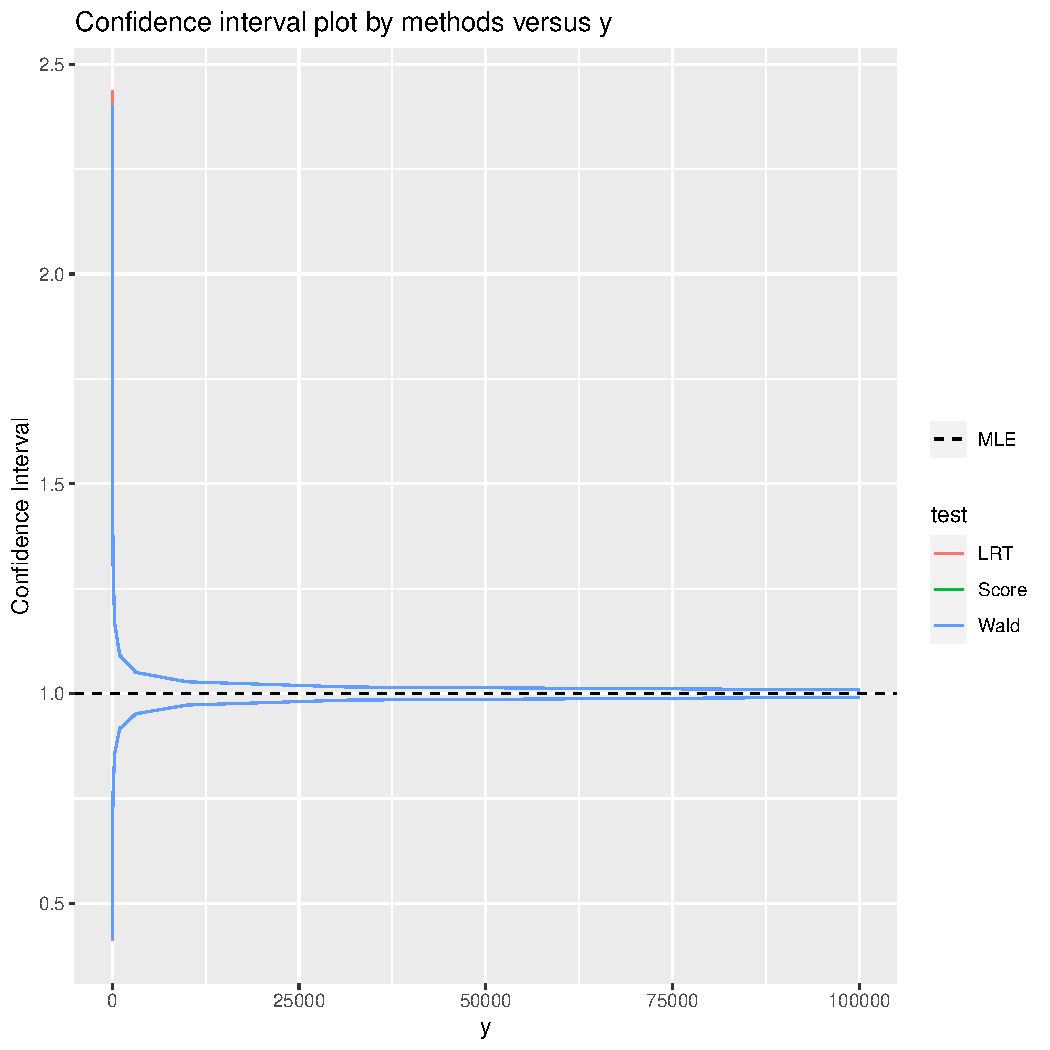
\includegraphics[width=\maxwidth]{unnamed-chunk-3-1} 
\end{knitrout}

\begin{knitrout}
\definecolor{shadecolor}{rgb}{0.969, 0.969, 0.969}\color{fgcolor}\begin{kframe}
\begin{alltt}
\hlcom{#try to plot on log(y) scale}
\hlstd{bdf}\hlopt{$}\hlstd{logy} \hlkwb{=} \hlkwd{log}\hlstd{(bdf}\hlopt{$}\hlstd{y)}
\hlstd{bdf} \hlopt \hlkwd{ggplot}\hlstd{(}\hlkwd{aes}\hlstd{(}\hlkwc{color}\hlstd{=test))} \hlopt{+}
  \hlkwd{geom_line}\hlstd{(}\hlkwd{aes}\hlstd{(}\hlkwc{x}\hlstd{=logy,} \hlkwc{y}\hlstd{=lower))}\hlopt{+}
  \hlkwd{geom_line}\hlstd{(}\hlkwd{aes}\hlstd{(}\hlkwc{x}\hlstd{=logy,} \hlkwc{y}\hlstd{=upper))}\hlopt{+}
  \hlkwd{geom_hline}\hlstd{(}\hlkwd{aes}\hlstd{(}\hlkwc{yintercept}\hlstd{=}\hlnum{1}\hlstd{,} \hlkwc{linetype}\hlstd{=}\hlstr{"MLE"}\hlstd{))}\hlopt{+}
  \hlkwd{scale_linetype_manual}\hlstd{(}\hlkwc{name} \hlstd{=} \hlstr{""}\hlstd{,} \hlkwc{values}\hlstd{=}\hlnum{2}\hlstd{)}\hlopt{+}
  \hlkwd{ggtitle}\hlstd{(}\hlstr{"Confidence interval plot by methods versus log(y)"}\hlstd{)}\hlopt{+}
  \hlkwd{labs}\hlstd{(}\hlkwc{x}\hlstd{=}\hlstr{"log(y)"}\hlstd{,} \hlkwc{y}\hlstd{=}\hlstr{"Confidence Interval"}\hlstd{)}
\end{alltt}
\end{kframe}
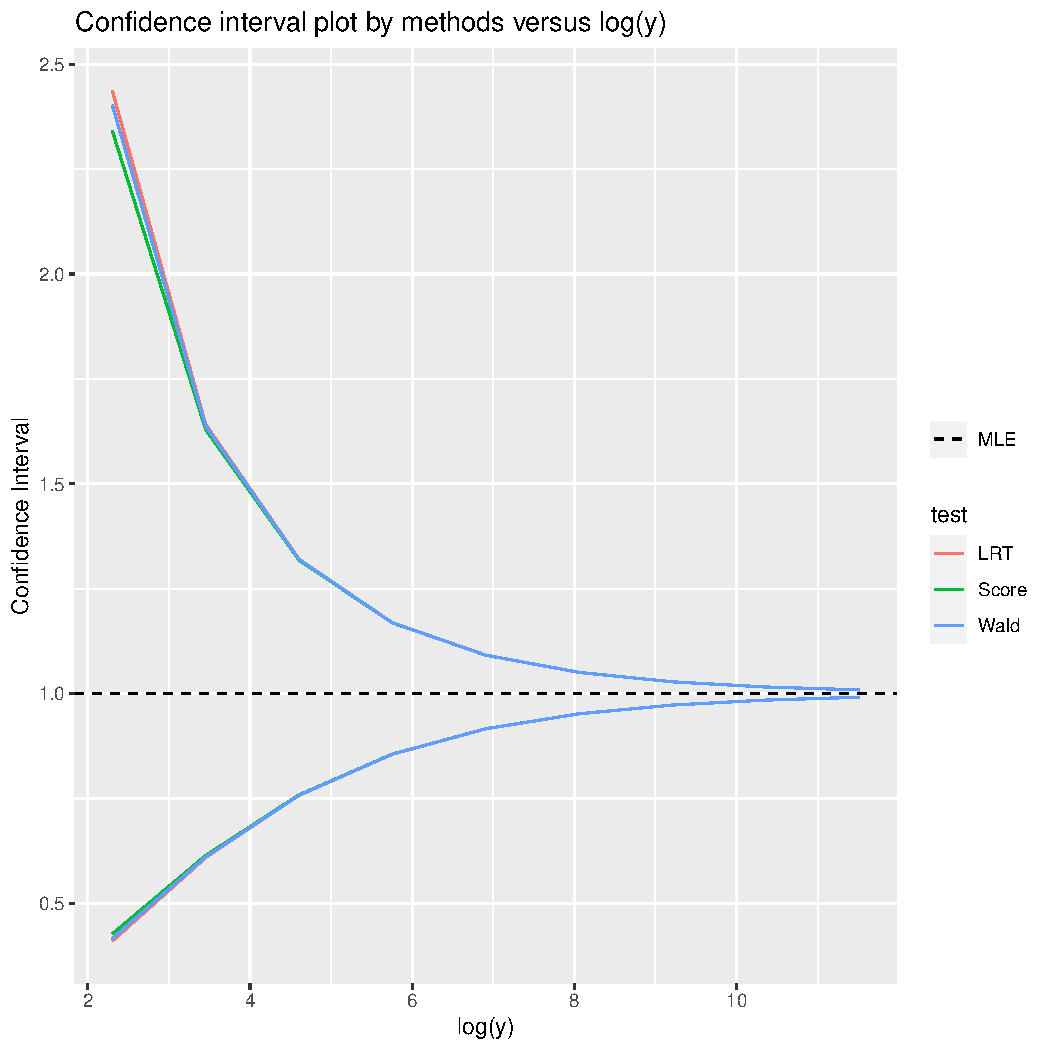
\includegraphics[width=\maxwidth]{unnamed-chunk-4-1} 
\end{knitrout}

Due to the nature of exponential function, the lower endpoints of three intervals differ only extremely slightly. The upper endpoints of three intervals also differ quite slightly, with LRT giving the widest confidence interval and score test inverted CI giving the most narrowest. As $y$ increases, three confidence intervals all become narrow converging to 1, which is the MLE for $e^{\beta_1}$.

\item[(c)]
\begin{knitrout}
\definecolor{shadecolor}{rgb}{0.969, 0.969, 0.969}\color{fgcolor}\begin{kframe}
\begin{alltt}
\hlstd{alpha} \hlkwb{=} \hlnum{0.05}
\hlstd{muval} \hlkwb{=} \hlkwd{c}\hlstd{(}\hlnum{10}\hlopt{^}\hlkwd{seq}\hlstd{(}\hlnum{1}\hlstd{,}\hlnum{5}\hlstd{,}\hlnum{0.5}\hlstd{))}
\hlstd{cmudf} \hlkwb{=} \hlkwd{data.frame}\hlstd{()}
\hlkwa{for} \hlstd{(i} \hlkwa{in} \hlnum{1}\hlopt{:}\hlkwd{length}\hlstd{(muval))\{}
  \hlstd{mu} \hlkwb{=} \hlstd{muval[i]}
  \hlstd{totalsample} \hlkwb{=} \hlkwd{rpois}\hlstd{(}\hlnum{10000}\hlstd{,mu)}
  \hlcom{#get random (y1,y2)}
  \hlstd{yone} \hlkwb{=} \hlstd{totalsample[}\hlnum{1}\hlopt{:}\hlnum{5000}\hlstd{]}
  \hlstd{ytwo} \hlkwb{=} \hlstd{totalsample[}\hlnum{5001}\hlopt{:}\hlnum{10000}\hlstd{]}
  \hlstd{dfloop} \hlkwb{=} \hlkwd{data.frame}\hlstd{()}
  \hlkwa{for} \hlstd{(j} \hlkwa{in} \hlnum{1}\hlopt{:}\hlnum{5000}\hlstd{)\{}
    \hlcom{#wald}
    \hlstd{dftemp} \hlkwb{=} \hlkwd{get_ci_wald}\hlstd{(yone[j],ytwo[j],alpha)}
    \hlstd{dftemp}\hlopt{$}\hlstd{test} \hlkwb{=} \hlstr{"Wald"}
    \hlstd{dftemp}\hlopt{$}\hlstd{mu} \hlkwb{=} \hlstd{mu}
    \hlstd{dftemp}\hlopt{$}\hlstd{contained} \hlkwb{=} \hlstd{(dftemp}\hlopt{$}\hlstd{lower} \hlopt{<=} \hlnum{1} \hlopt{&&} \hlstd{dftemp}\hlopt{$}\hlstd{upper} \hlopt{>=}\hlnum{1}\hlstd{)}
    \hlstd{dftemp}\hlopt{$}\hlstd{length} \hlkwb{=} \hlstd{dftemp}\hlopt{$}\hlstd{upper} \hlopt{-} \hlstd{dftemp}\hlopt{$}\hlstd{lower}
    \hlstd{dfloop} \hlkwb{=} \hlkwd{rbind}\hlstd{(dfloop, dftemp)}
    \hlcom{#score}
    \hlstd{dftemp} \hlkwb{=} \hlkwd{get_ci_score}\hlstd{(yone[j],ytwo[j],alpha)}
    \hlstd{dftemp}\hlopt{$}\hlstd{test} \hlkwb{=} \hlstr{"Score"}
    \hlstd{dftemp}\hlopt{$}\hlstd{mu} \hlkwb{=} \hlstd{mu}
    \hlstd{dftemp}\hlopt{$}\hlstd{contained} \hlkwb{=} \hlstd{(dftemp}\hlopt{$}\hlstd{lower} \hlopt{<=} \hlnum{1} \hlopt{&&} \hlstd{dftemp}\hlopt{$}\hlstd{upper} \hlopt{>=}\hlnum{1}\hlstd{)}
    \hlstd{dftemp}\hlopt{$}\hlstd{length} \hlkwb{=} \hlstd{dftemp}\hlopt{$}\hlstd{upper} \hlopt{-} \hlstd{dftemp}\hlopt{$}\hlstd{lower}
    \hlstd{dfloop} \hlkwb{=} \hlkwd{rbind}\hlstd{(dfloop, dftemp)}
    \hlcom{#lrt}
    \hlstd{dftemp} \hlkwb{=} \hlkwd{get_ci_lrt}\hlstd{(yone[j],ytwo[j],alpha)}
    \hlstd{dftemp}\hlopt{$}\hlstd{test} \hlkwb{=} \hlstr{"LRT"}
    \hlstd{dftemp}\hlopt{$}\hlstd{mu} \hlkwb{=} \hlstd{mu}
    \hlstd{dftemp}\hlopt{$}\hlstd{contained} \hlkwb{=} \hlstd{(dftemp}\hlopt{$}\hlstd{lower} \hlopt{<=} \hlnum{1} \hlopt{&&} \hlstd{dftemp}\hlopt{$}\hlstd{upper} \hlopt{>=}\hlnum{1}\hlstd{)}
    \hlstd{dftemp}\hlopt{$}\hlstd{length} \hlkwb{=} \hlstd{dftemp}\hlopt{$}\hlstd{upper} \hlopt{-} \hlstd{dftemp}\hlopt{$}\hlstd{lower}
    \hlstd{dfloop} \hlkwb{=} \hlkwd{rbind}\hlstd{(dfloop, dftemp)}
  \hlstd{\}}
  \hlcom{#get rid of the inifnity}
  \hlstd{dfloop} \hlkwb{=} \hlstd{dfloop[}\hlkwd{is.finite}\hlstd{(dfloop}\hlopt{$}\hlstd{lower),]}
  \hlstd{cmudf} \hlkwb{=} \hlkwd{rbind}\hlstd{(cmudf,}
                \hlkwd{data.frame}\hlstd{(dfloop} \hlopt \hlkwd{group_by}\hlstd{(test,mu)} \hlopt
                          \hlkwd{summarise_at}\hlstd{(}\hlkwd{vars}\hlstd{(lower, upper, length, contained),}
                                        \hlkwd{list}\hlstd{(}\hlkwc{name}\hlstd{=mean))))}

\hlstd{\}}
\hlkwd{require}\hlstd{(latex2exp)}
\hlcom{#plot the average coverage}
\hlstd{cmudf} \hlopt \hlkwd{ggplot}\hlstd{(}\hlkwd{aes}\hlstd{(}\hlkwc{fill}\hlstd{=test,} \hlkwc{color}\hlstd{=test))}\hlopt{+}
  \hlkwd{geom_line}\hlstd{(}\hlkwd{aes}\hlstd{(}\hlkwc{x}\hlstd{=mu,} \hlkwc{y}\hlstd{=contained_name))}\hlopt{+}
  \hlkwd{ggtitle}\hlstd{(}\hlkwd{TeX}\hlstd{(}\hlstr{"Average coverage plot by methods versus $\textbackslash{}\textbackslash{}mu$"}\hlstd{))}\hlopt{+}
  \hlkwd{labs}\hlstd{(}\hlkwc{x}\hlstd{=}\hlkwd{TeX}\hlstd{(}\hlstr{"$\textbackslash{}\textbackslash{}mu$"}\hlstd{),} \hlkwc{y}\hlstd{=}\hlstr{"Average coverage"}\hlstd{)}
\end{alltt}
\end{kframe}
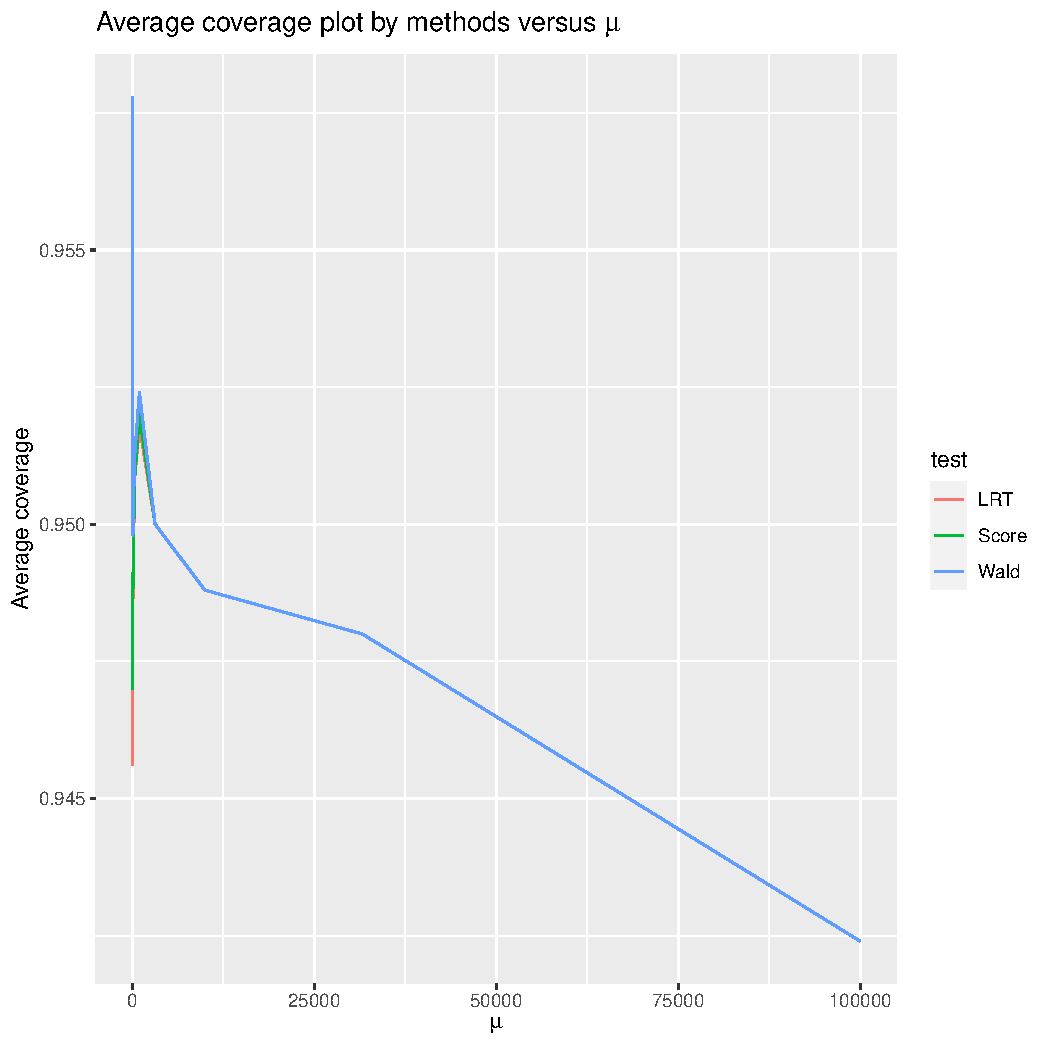
\includegraphics[width=\maxwidth]{unnamed-chunk-5-1} 
\begin{kframe}\begin{alltt}
\hlcom{#plot the average length}
\hlstd{cmudf} \hlopt \hlkwd{ggplot}\hlstd{(}\hlkwd{aes}\hlstd{(}\hlkwc{fill}\hlstd{=test,} \hlkwc{color}\hlstd{= test))} \hlopt{+}
  \hlkwd{geom_line}\hlstd{(}\hlkwd{aes}\hlstd{(}\hlkwc{x}\hlstd{=mu,} \hlkwc{y}\hlstd{=length_name))}\hlopt{+}
  \hlkwd{ggtitle}\hlstd{(}\hlkwd{TeX}\hlstd{(}\hlstr{"Average intereval length by methods versus $\textbackslash{}\textbackslash{}mu$"}\hlstd{))}\hlopt{+}
  \hlkwd{labs}\hlstd{(}\hlkwc{x}\hlstd{=}\hlkwd{TeX}\hlstd{(}\hlstr{"$\textbackslash{}\textbackslash{}mu$"}\hlstd{),} \hlkwc{y}\hlstd{=}\hlstr{"Average Interval Length"}\hlstd{)}
\end{alltt}
\end{kframe}
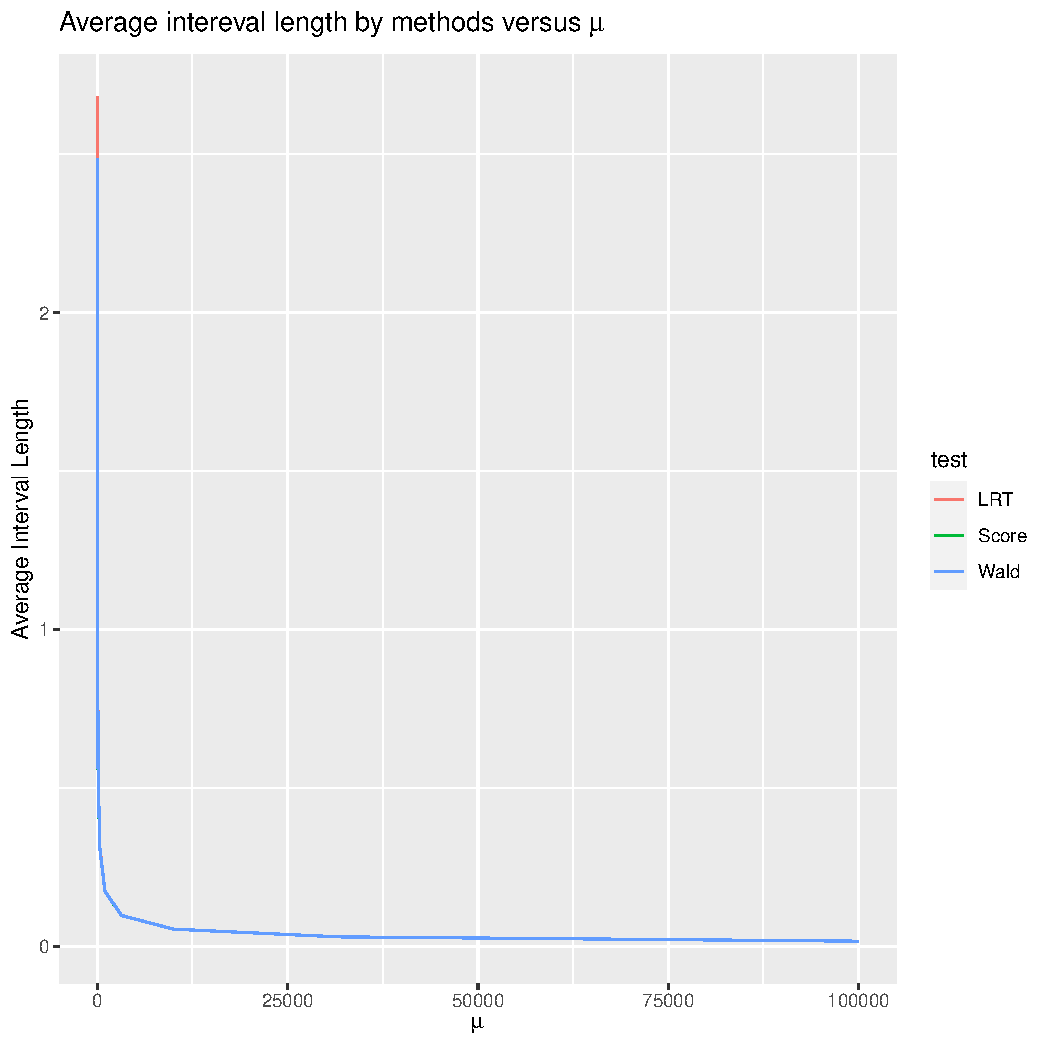
\includegraphics[width=\maxwidth]{unnamed-chunk-5-2} 
\end{knitrout}

\begin{knitrout}
\definecolor{shadecolor}{rgb}{0.969, 0.969, 0.969}\color{fgcolor}\begin{kframe}
\begin{alltt}
\hlcom{#try to plot the average coverage on log(mu) scale}
\hlstd{cmudf}\hlopt{$}\hlstd{logmu} \hlkwb{=} \hlkwd{log}\hlstd{(cmudf}\hlopt{$}\hlstd{mu)}
\hlstd{cmudf} \hlopt \hlkwd{ggplot}\hlstd{(}\hlkwd{aes}\hlstd{(}\hlkwc{fill}\hlstd{=test,} \hlkwc{color}\hlstd{= test))} \hlopt{+}
  \hlkwd{geom_line}\hlstd{(}\hlkwd{aes}\hlstd{(}\hlkwc{x}\hlstd{=logmu,} \hlkwc{y}\hlstd{=contained_name))}\hlopt{+}
  \hlkwd{ggtitle}\hlstd{(}\hlkwd{TeX}\hlstd{(}\hlstr{"Average coverage plot by methods versus $\textbackslash{}\textbackslash{}log(\textbackslash{}\textbackslash{}mu)$"}\hlstd{))}\hlopt{+}
  \hlkwd{labs}\hlstd{(}\hlkwc{x}\hlstd{=}\hlkwd{TeX}\hlstd{(}\hlstr{"$\textbackslash{}\textbackslash{}log(\textbackslash{}\textbackslash{}mu)$"}\hlstd{),} \hlkwc{y}\hlstd{=}\hlstr{"Average coverage"}\hlstd{)}
\end{alltt}
\end{kframe}
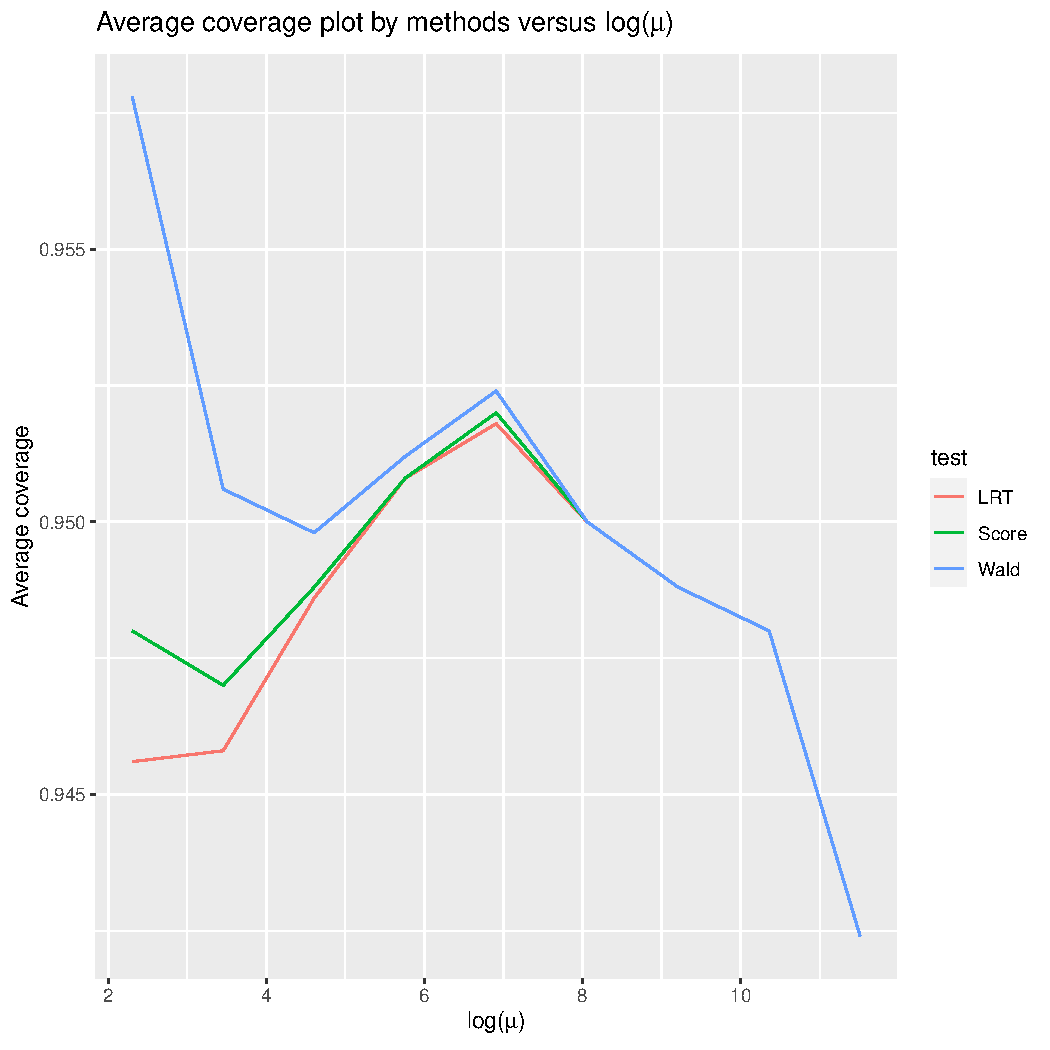
\includegraphics[width=\maxwidth]{unnamed-chunk-6-1} 
\begin{kframe}\begin{alltt}
\hlcom{#plot the average length on log(mu) scale}
\hlstd{cmudf} \hlopt \hlkwd{ggplot}\hlstd{(}\hlkwd{aes}\hlstd{(}\hlkwc{fill}\hlstd{=test,} \hlkwc{color}\hlstd{= test))} \hlopt{+}
  \hlkwd{geom_line}\hlstd{(}\hlkwd{aes}\hlstd{(}\hlkwc{x}\hlstd{=logmu,} \hlkwc{y}\hlstd{=length_name))}\hlopt{+}
  \hlkwd{ggtitle}\hlstd{(}\hlkwd{TeX}\hlstd{(}\hlstr{"Average intereval length by methods versus $\textbackslash{}\textbackslash{}log(\textbackslash{}\textbackslash{}mu)$"}\hlstd{))}\hlopt{+}
  \hlkwd{labs}\hlstd{(}\hlkwc{x}\hlstd{=}\hlkwd{TeX}\hlstd{(}\hlstr{"$\textbackslash{}\textbackslash{}log(\textbackslash{}\textbackslash{}mu)$"}\hlstd{),} \hlkwc{y}\hlstd{=}\hlstr{"Average Interval Length"}\hlstd{)}
\end{alltt}
\end{kframe}
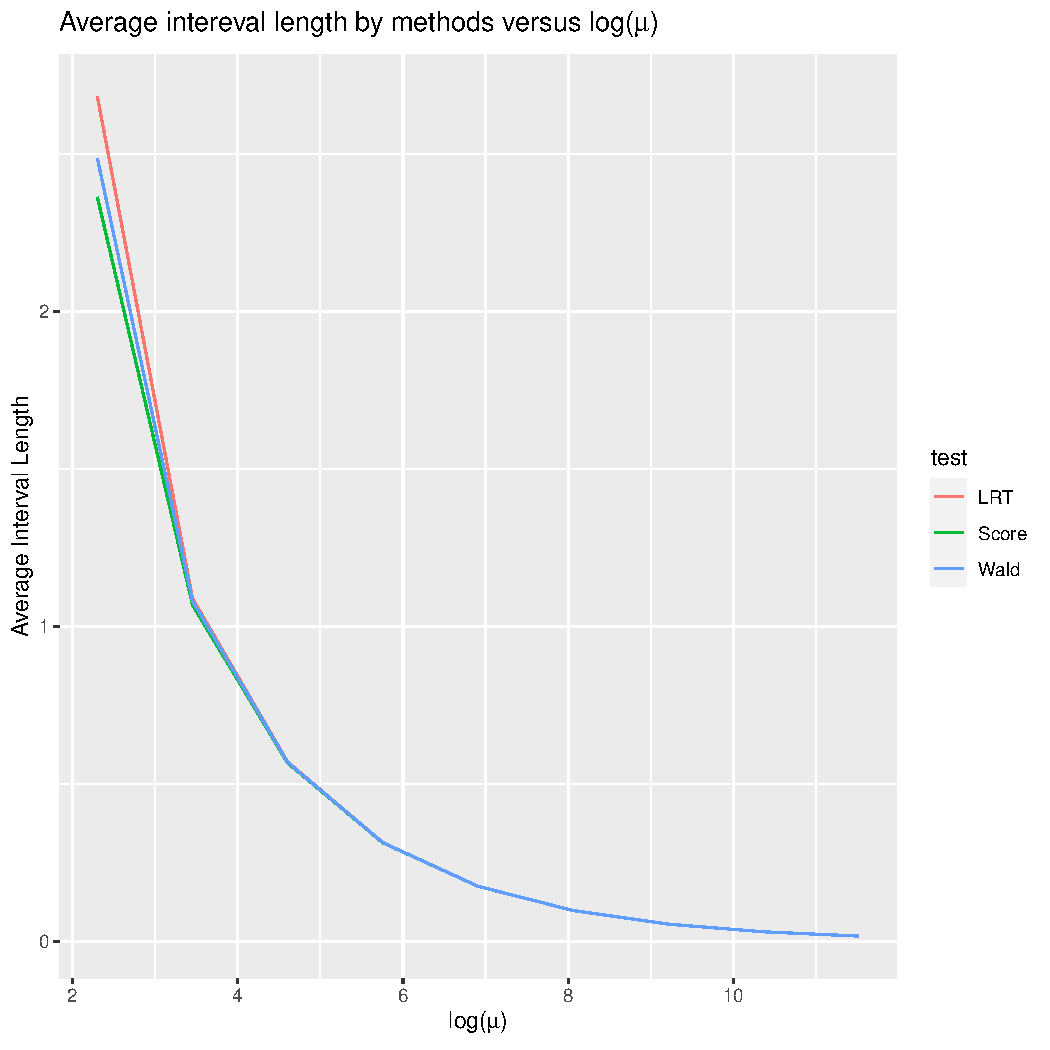
\includegraphics[width=\maxwidth]{unnamed-chunk-6-2} 
\end{knitrout}

LRT has the worst coverage while Walds has the best among all three methods when $\mu$ is not very large. However, also notice that the difference in coverage between three methods are not significant (at most less than 2\%). It can be said that the difference in the coverage between three methods is negligible. LRT yields the highest average confidence length while score test yields the lowest among all three methods, while this difference, as can be seen in the graph, is also negligible when $\mu_1,\mu_2$ is not too small. As expected, when $\mu_1,\mu_2$ increases, the coverage of three confidence intervals become increasingly similar and the confidence interval lengths all become narrower.

\item[(d)]
I think score test is good.

\begin{knitrout}
\definecolor{shadecolor}{rgb}{0.969, 0.969, 0.969}\color{fgcolor}\begin{kframe}
\begin{alltt}
\hlcom{#use score test}
\hlkwd{get_ci_score}\hlstd{(}\hlnum{60}\hlstd{,}\hlnum{90}\hlstd{,}\hlnum{.05}\hlstd{)}
\end{alltt}
\begin{verbatim}
##      lower    upper
## 1 1.083547 2.076514
\end{verbatim}
\end{kframe}
\end{knitrout}

The confidence interval for $e^{\beta_1}$ does not contain 1, which means $\beta_1=0$ is not included. We reject the null hypothesis $\beta_1=0$, meaning that it is not very possible that two inboxes receive emails at the same rate.

\end{enumerate}
\end{sol}


\begin{prob} \label{prob:blocks-data}\textbf{Case study: Child development.} \\

\noindent Children were asked to build towers as high as they could out of cubical and cylindrical blocks.\footnote{Johnson, B., Courtney, D.M.: Tower building. Child Development 2(2), 161-162 (1931).} The number of blocks used and the time taken were recorded (see \verb|blocks_data| below). In this problem, only consider the number of blocks used and the age of the child.
\begin{knitrout}
\definecolor{shadecolor}{rgb}{0.969, 0.969, 0.969}\color{fgcolor}\begin{kframe}
\begin{alltt}
\hlstd{blocks_data} \hlkwb{=} \hlkwd{read_tsv}\hlstd{(}\hlstr{"../../data/blocks.tsv"}\hlstd{)}
\hlkwd{print}\hlstd{(blocks_data,} \hlkwc{n} \hlstd{=} \hlnum{5}\hlstd{)}
\end{alltt}
\begin{verbatim}
## # A tibble: 100 x 6
##   Child Number  Time Trial Shape   Age
##   <chr>  <dbl> <dbl> <dbl> <chr> <dbl>
## 1 A         11  30       1 Cube   4.67
## 2 B          9  19       1 Cube   5   
## 3 C          8  18.6     1 Cube   4.42
## 4 D          9  23       1 Cube   4.33
## 5 E         10  29       1 Cube   4.33
## # ... with 95 more rows
\end{verbatim}
\end{kframe}
\end{knitrout}

\begin{enumerate}

\item[(a)] Create a scatter plot of blocks used versus age; since there are exact duplicates of \verb|(Number, Age)| in the data, use \verb|geom_count()| instead of \verb|geom_point()|. Propose a GLM to model the number of blocks used as a function of age.

\item[(b)] Fit this GLM using R, and write down the fitted model. Determine the standard error for each regression parameter, and find the 95\% Wald confidence intervals for the regression coefficients.

\item[(c)] Use Wald, score, and likelihood ratio tests to determine if age seems necessary in the model. Compare the results and comment.

\item[(d)] Plot the number of blocks used against age as in part (a), adding the relationship described by the fitted model as well as lines indicating the lower and upper 95\% confidence intervals for these fitted values.

\end{enumerate}

\noindent \textit{Acknowledgment: This problem was drawn from ``Generalized Linear Models With Examples in R'' (Dunn and Smyth, 2018).}


\end{prob}

\begin{sol}
\begin{enumerate}
\item[(a)]
\begin{knitrout}
\definecolor{shadecolor}{rgb}{0.969, 0.969, 0.969}\color{fgcolor}\begin{kframe}
\begin{alltt}
\hlcom{#plot the data}
\hlkwd{ggplot}\hlstd{(blocks_data,}\hlkwd{aes}\hlstd{(}\hlkwc{y}\hlstd{=Number,}\hlkwc{x}\hlstd{=Age))} \hlopt{+}
  \hlkwd{geom_count}\hlstd{()}\hlopt{+}
  \hlkwd{ggtitle}\hlstd{(}\hlstr{"Count plot versus age"}\hlstd{)}\hlopt{+}
  \hlkwd{labs}\hlstd{(}\hlkwc{y}\hlstd{=}\hlstr{"Number of blocks"}\hlstd{)}
\end{alltt}
\end{kframe}
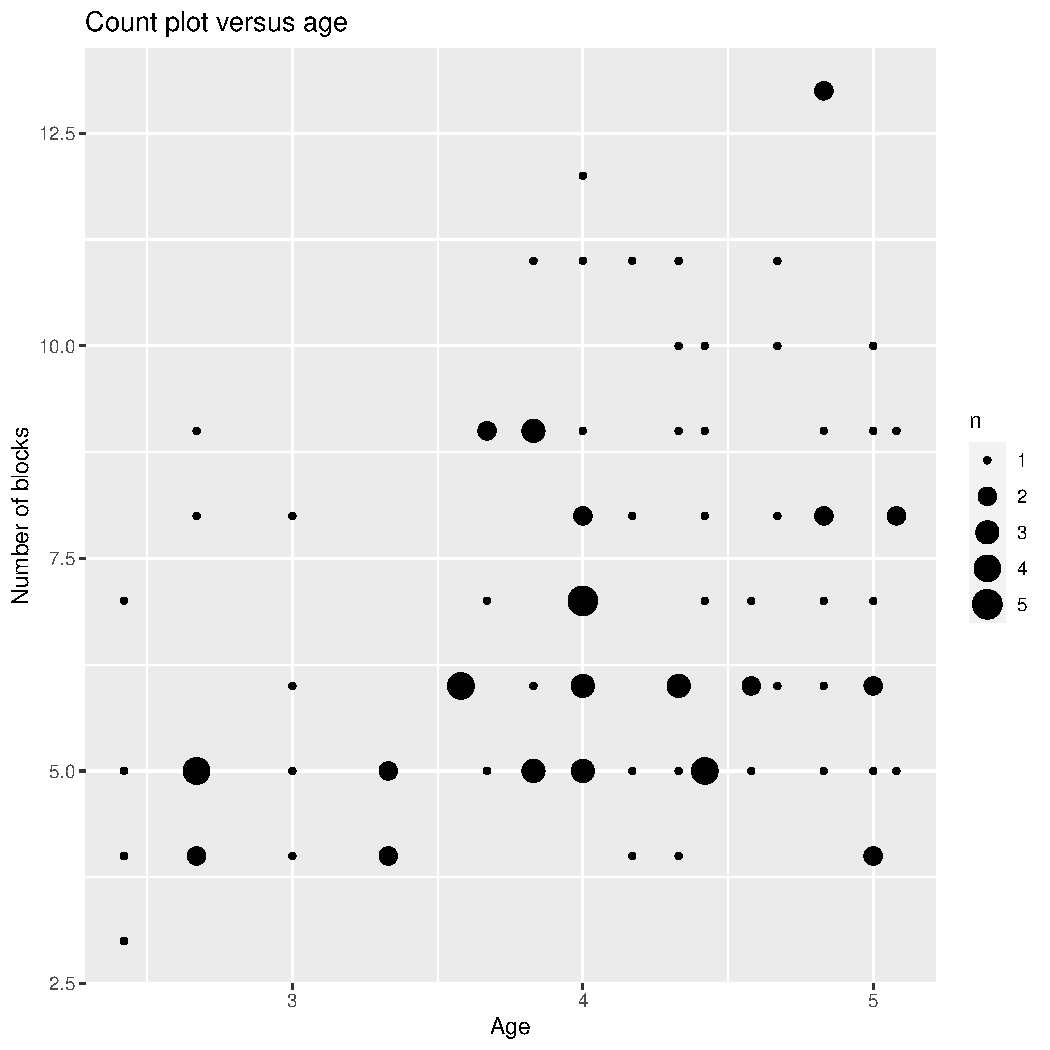
\includegraphics[width=\maxwidth]{unnamed-chunk-9-1} 
\end{knitrout}
\item[(b)]
\begin{knitrout}
\definecolor{shadecolor}{rgb}{0.969, 0.969, 0.969}\color{fgcolor}\begin{kframe}
\begin{alltt}
\hlcom{#run glm}
\hlkwd{require}\hlstd{(MASS)}
\hlstd{glmvar} \hlkwb{=} \hlstd{blocks_data} \hlopt
  \hlkwd{glm}\hlstd{(}\hlkwc{formula} \hlstd{= Number}\hlopt{~}\hlstd{Age,} \hlkwc{family} \hlstd{=} \hlkwd{poisson}\hlstd{(}\hlkwc{link} \hlstd{=} \hlstr{"log"}\hlstd{))}
\hlstd{sumglmvar} \hlkwb{=} \hlkwd{summary}\hlstd{(glmvar)}
\hlstd{sumglmvar}
\end{alltt}
\begin{verbatim}
## 
## Call:
## glm(formula = Number ~ Age, family = poisson(link = "log"), data = .)
## 
## Deviance Residuals: 
##     Min       1Q   Median       3Q      Max  
## -1.4977  -0.6542  -0.1984   0.4714   1.8155  
## 
## Coefficients:
##             Estimate Std. Error z value Pr(>|z|)    
## (Intercept)   1.3447     0.2223   6.048 1.47e-09 ***
## Age           0.1415     0.0534   2.650  0.00805 ** 
## ---
## Signif. codes:  0 '***' 0.001 '**' 0.01 '*' 0.05 '.' 0.1 ' ' 1
## 
## (Dispersion parameter for poisson family taken to be 1)
## 
##     Null deviance: 69.429  on 99  degrees of freedom
## Residual deviance: 62.244  on 98  degrees of freedom
## AIC: 439.64
## 
## Number of Fisher Scoring iterations: 4
\end{verbatim}
\begin{alltt}
\hlcom{#print look at the std. error in coef}
\hlkwd{coef}\hlstd{(sumglmvar)}
\end{alltt}
\begin{verbatim}
##              Estimate Std. Error  z value     Pr(>|z|)
## (Intercept) 1.3446992 0.22235364 6.047570 1.470468e-09
## Age         0.1415096 0.05340039 2.649974 8.049803e-03
\end{verbatim}
\end{kframe}
\end{knitrout}


\begin{knitrout}
\definecolor{shadecolor}{rgb}{0.969, 0.969, 0.969}\color{fgcolor}\begin{kframe}
\begin{alltt}
\hlcom{#get Wald CI}
\hlkwd{confint.default}\hlstd{(glmvar)}
\end{alltt}
\begin{verbatim}
##                  2.5 %    97.5 %
## (Intercept) 0.90889409 1.7805044
## Age         0.03684679 0.2461725
\end{verbatim}
\end{kframe}
\end{knitrout}

\item[(c)]
\begin{knitrout}
\definecolor{shadecolor}{rgb}{0.969, 0.969, 0.969}\color{fgcolor}\begin{kframe}
\begin{alltt}
\hlcom{#create a null model}
\hlstd{qqglmvar} \hlkwb{=} \hlkwd{glm}\hlstd{(Number}\hlopt{~}\hlnum{1}\hlstd{,} \hlkwc{data} \hlstd{= blocks_data,} \hlkwc{family} \hlstd{=} \hlkwd{poisson}\hlstd{(}\hlkwc{link} \hlstd{=} \hlstr{"log"}\hlstd{))}
\hlcom{#score test}
\hlkwd{anova}\hlstd{(qqglmvar,glmvar,}\hlkwc{test}\hlstd{=}\hlstr{"Rao"}\hlstd{)}
\end{alltt}
\begin{verbatim}
## Analysis of Deviance Table
## 
## Model 1: Number ~ 1
## Model 2: Number ~ Age
##   Resid. Df Resid. Dev Df Deviance    Rao Pr(>Chi)   
## 1        99     69.429                               
## 2        98     62.244  1   7.1854 7.0346 0.007995 **
## ---
## Signif. codes:  0 '***' 0.001 '**' 0.01 '*' 0.05 '.' 0.1 ' ' 1
\end{verbatim}
\begin{alltt}
\hlcom{#likelihood ratio test}
\hlkwd{anova}\hlstd{(qqglmvar,glmvar,}\hlkwc{test}\hlstd{=}\hlstr{"LRT"}\hlstd{)}
\end{alltt}
\begin{verbatim}
## Analysis of Deviance Table
## 
## Model 1: Number ~ 1
## Model 2: Number ~ Age
##   Resid. Df Resid. Dev Df Deviance Pr(>Chi)   
## 1        99     69.429                        
## 2        98     62.244  1   7.1854  0.00735 **
## ---
## Signif. codes:  0 '***' 0.001 '**' 0.01 '*' 0.05 '.' 0.1 ' ' 1
\end{verbatim}
\begin{alltt}
\hlcom{#wald test}
\hlkwd{coef}\hlstd{(sumglmvar)}
\end{alltt}
\begin{verbatim}
##              Estimate Std. Error  z value     Pr(>|z|)
## (Intercept) 1.3446992 0.22235364 6.047570 1.470468e-09
## Age         0.1415096 0.05340039 2.649974 8.049803e-03
\end{verbatim}
\end{kframe}
\end{knitrout}

We observe that age is necessary with very small p values throughout all three tests. Wald test gives a slightly higher p value, which makes sense because 100 is not a very large number while Wald test performs slightly worse for small samples. On the other hand, the difference in p value is indeed not very large from other two tests because 100 is not too small either. LRT's p-value is smaller than Wald's and score test's even though the difference is insignificant too. 


\item[(d)]
\begin{knitrout}
\definecolor{shadecolor}{rgb}{0.969, 0.969, 0.969}\color{fgcolor}\begin{kframe}
\begin{alltt}
\hlcom{#plot count + fitted value + 95% CI}
\hlstd{newdata} \hlkwb{=} \hlkwd{data.frame}\hlstd{(}\hlkwc{Age}\hlstd{=blocks_data}\hlopt{$}\hlstd{Age)}
\hlstd{preds} \hlkwb{=} \hlkwd{predict}\hlstd{(glmvar, newdata,} \hlkwc{se.fit}\hlstd{=}\hlnum{TRUE}\hlstd{,}\hlkwc{interval}\hlstd{=}\hlstr{'confidence'}\hlstd{)}
\hlstd{blocks_data}\hlopt{$}\hlstd{lowerCI} \hlkwb{=} \hlkwd{exp}\hlstd{(preds}\hlopt{$}\hlstd{fit} \hlopt{-} \hlnum{1.96}\hlopt{*}\hlstd{preds}\hlopt{$}\hlstd{se.fit)}
\hlstd{blocks_data}\hlopt{$}\hlstd{upperCI} \hlkwb{=} \hlkwd{exp}\hlstd{(preds}\hlopt{$}\hlstd{fit} \hlopt{+} \hlnum{1.96}\hlopt{*}\hlstd{preds}\hlopt{$}\hlstd{se.fit)}
\hlstd{blocks_data}\hlopt{$}\hlstd{fitdata} \hlkwb{=} \hlkwd{exp}\hlstd{(preds}\hlopt{$}\hlstd{fit)}

\hlstd{blocks_data} \hlopt \hlkwd{ggplot}\hlstd{(}\hlkwd{aes}\hlstd{(}\hlkwc{y}\hlstd{=Number,}\hlkwc{x}\hlstd{=Age))} \hlopt{+}
  \hlkwd{geom_count}\hlstd{()}\hlopt{+}
  \hlkwd{geom_ribbon}\hlstd{(}\hlkwd{aes}\hlstd{(}\hlkwc{ymin} \hlstd{= lowerCI,} \hlkwc{ymax} \hlstd{= upperCI),}\hlkwc{fill}\hlstd{=}\hlstr{"#FFF03388"}\hlstd{)}\hlopt{+}
  \hlkwd{geom_line}\hlstd{(}\hlkwd{aes}\hlstd{(}\hlkwc{y}\hlstd{=fitdata),}\hlkwc{color}\hlstd{=}\hlstr{"red"}\hlstd{)}\hlopt{+}
  \hlkwd{ggtitle}\hlstd{(}\hlstr{"Count plot versus age with 95% CI and fitted value"}\hlstd{)}\hlopt{+}
  \hlkwd{labs}\hlstd{(}\hlkwc{y}\hlstd{=}\hlstr{"Number of blocks"}\hlstd{)}
\end{alltt}
\end{kframe}
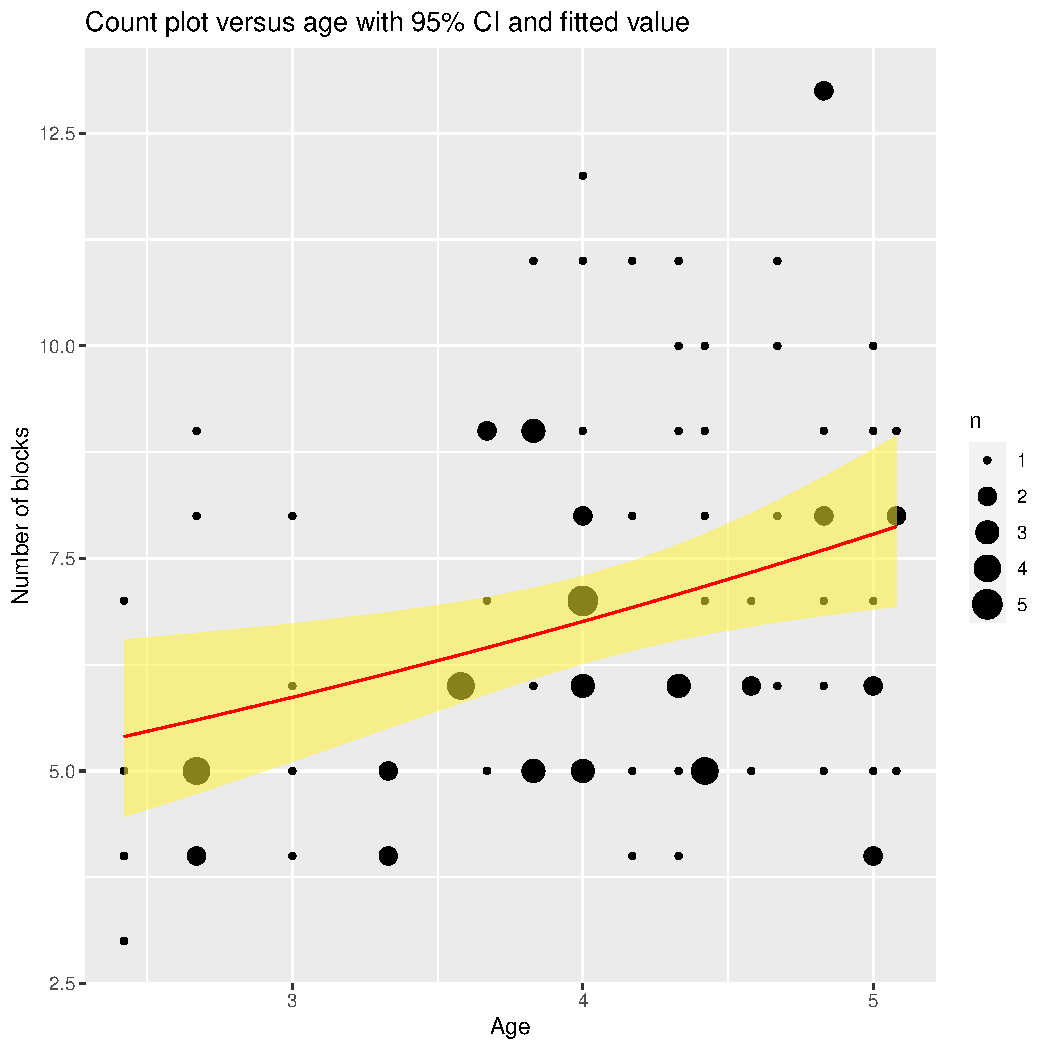
\includegraphics[width=\maxwidth]{unnamed-chunk-13-1} 
\end{knitrout}

\end{enumerate}

\end{sol}


\end{document}
